\chapter[第三章]{} % (fold)
\label{cha:chapter3}

\section{3次样条插值函数}

\subsection{问题}

\begin{enumerate}[(1)]
    \item 编制求第一型3次样条插值函数的通用程序;
    \item 已知汽车门曲线型值点的数据如下:

        \begin{table}[ht]\centering
        \begin{tabular}{c|cccccccccccc}
            i & 0 & 1 & 2 & 3 & 4 & 5 & 6 & 7 & 8 & 9 & 10\\
            \hline
            $x_i$ & 0 & 1 & 2 & 3 & 4 & 5 & 6 & 7 & 8 & 9 & 10\\
            $y_i$ & 2.51 & 3.30 & 4.04 & 4.70 & 5.22 & 5.54 & 5.78 & 5.40 & 5.57 & 5.70 & 5.80 
        \end{tabular}
        \end{table}
    
    端点条件为$y_0^{'}=0.8$,$y_{10}^{'}=0.2$,用所编程序求车门的三次样条插值函数$S(x)$,并打印出$S(i+0.5),i=0,1,\cdots,9$。     
\end{enumerate}

\subsection{分析}

根据3次样条插值的定义,插值函数 $S(x)$ 满足:1. $S(x)$ 在每一个小区间上式3次多项式,2. $S(x)$ 在区间 $[a,b]$ 上具有连续2阶导数,3. $S(x)$ 经过每一个给定的插值节点。

在区间 $[a,b]$ 上有 $n+1$ 个插值节点,因此可以设每个小区间上的插值函数 $S_i(x)$ 为:

\begin{equation}
    S_i(x) = a_ix^3  + b_ix^2 + c_ix + d_i
\end{equation}

在 $n$ 个区间上有 $n$ 个插值函数,每个插值函数有 4 个参数,因此需要 $4n$ 个不相关的方程来求解:

\begin{enumerate}[(1)]
    \item 每个插值函数都会经过它所在小区间上的插值节点,即小区间的两个端点,有 $2n$ 个方程:
    \begin{align}
        S_i(x_i) &= y_i, \quad i \in [0,n-1] \\
        S_i(x_{i+1}) &= y_{i+1}, \quad i \in [0,n-1]
    \end{align}

    \item 一阶导数连续,即两个相邻的插值函数连接点处的一阶导数相等,有 $n-1$ 个方程:
    \begin{equation}
        S_i^{'}(x_{i+1}) = S_{i+1}^{'}(x_{i+1}), \quad i \in [0,n-2]
    \end{equation}

    \item 二阶导数连续,即两个相邻的插值函数连接点处的二阶导数相等,有 $n-1$ 个方程:
    \begin{equation}
        S_i^{''}(x_{i+1}) = S_{i+1}^{''}(x_{i+1}), \quad i \in [0,n-2]
    \end{equation}
    
    \item 第一型边界条件,已知两个端点处的一阶导数值,有 2 个方程:
    \begin{align}
        S_0^{'}(x_0) &= y_0^{'} \\
        S_{n-1}^{'}(x_n) &= y_n^{'}
    \end{align}
\end{enumerate}

$4n$ 个方程,使用列主元高斯法求解方程,得到最终的插值函数。

\subsection{程序}

\begin{lstlisting}[style = python]
    import numpy as np
    import matplotlib.pyplot as plt
    from pylab import mpl
    import sys, os
    
    '''
    description: 
    param {*} x n+1 个插值点
    param {*} y n+1 个插值点
    return {*} n
    '''
    def Prejudgment(x, y):
        n1 = len(x)
        n2 = len(y)
        if n1 != n2:
            print('x 与 y 长度不相等')
            sys.exit()
        
        n = n1-1
        return n
            
    '''
    description: 求三次样条差值的 4n 个方程
    param: {x[0,n], y[0,n]} n+1 个插值点
    param: Type 三次样条边界条件 1 or 2 or 3
    return {A, B} [a0 b0 c0 d0 a1 b1 c1 d1 ... a(n-1) b(n-1) c(n-1) d(n-1)] = [B] 形式的方程组 
    '''
    def calculateEquationParameters(x, y, Type=1, dy0=0, dyn=0):
        n = Prejudgment(x, y)
    
        parameterA = []
        parameterB = []
        
        # S_i(x_i) = y_i
        # S_i(x_{i+1}) = y_{i+1}
        # 0 <= i <= n-1
        for i in range(0, n):
            # S_i(x_i) = y_i
            data = np.zeros(n*4)
            data[i*4] = pow(x[i], 3)
            data[i*4+1] = pow(x[i], 2)
            data[i*4+2] = x[i]
            data[i*4+3] = 1
            parameterA.append(data.tolist())
            parameterB.append(y[i])
            
            # S_i(x_{i+1}) = y_{i+1}
            data1 = np.zeros(n*4)
            data1[i*4] = pow(x[(i+1)], 3)
            data1[i*4+1] = pow(x[(i+1)], 2)
            data1[i*4+2] = x[(i+1)]
            data1[i*4+3] = 1
            parameterA.append(data1.tolist())
            parameterB.append(y[i+1])
    
        # S'_i(x_{i+1}) = S'_{i+1}(x_{i+1})
        # 0 <= i <= n-2
        for i in range(0, n-1):
            data = np.zeros(n*4)
    
            data[i*4] = 3 * pow(x[i+1], 2)
            data[i*4+1] = 2 * x[i+1]
            data[i*4+2] = 1
    
            data[(i+1)*4] = -3 * pow(x[i+1], 2)
            data[(i+1)*4+1] = -2 * x[i+1]
            data[(i+1)*4+2] = -1
            
            parameterA.append(data.tolist())
            parameterB.append(0)
    
        # S''_i(x_{i+1}) = S''_{i+1}(x_{i+1})
        # 0 <= i <= n-2
        for i in range(0, n-1):
            data = np.zeros(n*4)
    
            data[i*4] = 6 * x[i+1]
            data[i*4+1] = 2
    
            data[(i+1)*4] = -6 * x[i+1]
            data[(i+1)*4+1] = -2
            
            parameterA.append(data.tolist())
            parameterB.append(0)
    
        if Type == 1:
            # S'_0(x_0) = y'_0
            data = np.zeros(n*4)
            data[0] = 3 * pow(x[0], 2)
            data[1] = 2 * x[0]
            data[2] = 1
            parameterA.append(data.tolist())
            parameterB.append(dy0)
    
            # S'_{n-1}(x_n) = y'_n
            data = np.zeros(n*4)
            data[(n-1)*4] = 3 * pow(x[n], 2)
            data[(n-1)*4+1] = 2 * x[n]
            data[(n-1)*4+2] = 1
    
            parameterA.append(data.tolist())
            parameterB.append(dyn)
        elif Type == 2:
            # S''(a) = S''(b) = 0
    
            # S''_0(x_0) = 0
            data = np.zeros(n*4)
            data[0] = 6 * x[0]
            data[1] = 2
            parameterA.append(data.tolist())
            parameterB.append(0)
    
            # S''_{n-1}(x_n) = 0
            data = np.zeros(n*4)
            data[(n-1)*4] = 6 * x[n]
            data[(n-1)*4+1] = 2
            parameterA.append(data.tolist())
            parameterB.append(0)
    
        elif Type == 3:
            # S'(a) = S'(b) and # S''(a) = S''(b)
            pass
        else:
            print('Error! Unknown "Type" Value!')
    
        return parameterA, parameterB
    
    """
    功能:根据所给参数,计算三次函数的函数值:
    参数:OriginalInterval为原始x的区间, parameters为二次函数的系数,x为自变量
    返回值:为函数的因变量
    """
    def calculate(OriginalInterval, paremeters, x):
        n = int(len(paremeters)/4)
        result=[]
        for data_x in x:
    
            Interval = 0
            if data_x <= OriginalInterval[0]:
                Interval = 0
            elif data_x >= OriginalInterval[-1]:
                Interval = n-1
            else:
                for i in range(0,n):
                    if data_x >= OriginalInterval[i] and data_x < OriginalInterval[i+1]:
                        Interval = i
                        break
    
            result.append(paremeters[Interval*4+0]*data_x*data_x*data_x+paremeters[Interval*4+1]*data_x*data_x+paremeters[Interval*4+2]*data_x+paremeters[Interval*4+3])
        return result
    
    """
    功能:将函数绘制成图像
    参数:data_x,data_y为离散的点.new_data_x,new_data_y为由拉格朗日插值函数计算的值。x为函数的预测值。
    返回值:空
    """
    def Draw(data_x,data_y,new_data_x,new_data_y, title):
            plt.plot(new_data_x, new_data_y, label="拟合曲线", color="black")
            plt.scatter(data_x,data_y, label="离散数据",color="red")
            mpl.rcParams['font.sans-serif'] = ['SimHei']
            mpl.rcParams['axes.unicode_minus'] = False
            plt.title("三次样条函数")
            plt.legend(loc="upper left")
            plt.savefig(os.path.join(os.path.dirname(os.path.abspath(__file__)), title+'.png'), dpi=300)
            plt.show()
    
    def PrintS(parameterX):
        n = int(len(parameterX)/4)
        print('S(x) = ')
        for i in range(0,n):
            print("%.6g & %.6g & %.6g & %.6g \\\\" % (parameterX[i*4], parameterX[i*4+1], parameterX[i*4+2], parameterX[i*4+3]))
        print('\n\n')
            
    def main():
        x = [0,    1,    2,    3,    4,    5,    6,    7,    8,    9,    10]
        y = [2.51, 3.30, 4.04, 4.70, 5.22, 5.54, 5.78, 5.40, 5.57, 5.70, 5.80]
        dy0 = 0.8
        dyn = 0.2  
        parameterA, parameterB = calculateEquationParameters(x, y, 1, dy0, dyn)
        parameterX = MGauss_Caculate(parameterA, parameterB)
    
        PrintS(parameterX)
    
        # 画图
        new_data_x = np.arange(x[0]-0.5, x[-1]+0.6, 0.1)
        new_data_y = calculate(x, parameterX, new_data_x)
        Draw(x, y, new_data_x, new_data_y, '三次样条插值')
    
        # 打印
        new_data_x = np.arange(0.5, 10.5, 1)
        new_data_y = calculate(x, parameterX, new_data_x)
        # f4_5 = calculate(parameterX[8:12], [4.5])
        print(new_data_x)
        for i,data in enumerate(new_data_y):
            print("%.6g & " % data)
    
    if __name__ == "__main__":
    
        # 获取当前文件路径
        current_path = os.path.abspath(__file__)
        sys.path.append(os.path.abspath(os.path.join(os.path.dirname(current_path), '../')))
        # print(sys.path)
        # 调用 chapter3 中的列主元高斯消去法
        from chapter3.q3 import MGauss_Caculate
    
        main()
\end{lstlisting}

\subsection{算例}

对题目中的数据进行三次样条插值:

\begin{table}[ht]\centering
    \begin{tabular}{c|cccccccccccc}
        i & 0 & 1 & 2 & 3 & 4 & 5 & 6 & 7 & 8 & 9 & 10\\
        \hline
        $x_i$ & 0 & 1 & 2 & 3 & 4 & 5 & 6 & 7 & 8 & 9 & 10\\
        $y_i$ & 2.51 & 3.30 & 4.04 & 4.70 & 5.22 & 5.54 & 5.78 & 5.40 & 5.57 & 5.70 & 5.80 
    \end{tabular}
\end{table}

得到的插值函数系数为:

$$
\begin{bmatrix}
    -0.00851404 & -0.00148596 & 0.8 & 2.51 \\
    -0.00445789 & -0.0136544 & 0.812168 & 2.50594 \\
    -0.00365441 & -0.0184753 & 0.82181 & 2.49952 \\
    -0.0409245 & 0.316955 & -0.184482 & 3.50581 \\
    0.107352 & -1.46237 & 6.93281 & -5.98391 \\
    -0.268485 & 4.17519 & -21.255 & 40.9958 \\
    0.426587 & -8.33611 & 53.8128 & -109.14 \\
    -0.267865 & 6.24739 & -48.2717 & 129.057 \\
    0.0548723 & -1.4983 & 13.6939 & -36.1842 \\
    0.0583759 & -1.5929 & 14.5453 & -38.7383 \\
\end{bmatrix}
$$

题目中要求的 $S(i+0.5),i=0,1,\cdots,9$ 值如表\ref{tab:Si}所示,插值函数的图像如图\ref{fig:spline}所示。

\begin{table}[ht]\centering
\caption{$S(i+0.5),i=0,1,\cdots,9$}
\label{tab:Si}
    \begin{tabular}{c|cccccccccccc}
        i & 0 & 1 & 2 & 3 & 4 \\
        \hline
        $x_i$ & 0.5 & 1.5 & 2.5 & 3.5 & 4.5 \\
        $S(x)$ & 2.90856 & 3.67843 & 4.38147 & 4.98819 & 5.38328 \\
        \hline\hline
        i & 5 & 6 & 7 & 8 & 9 \\
        \hline
        $x_i$ & 5.5 & 6.5 & 7.5 & 8.5 & 9.5\\
        $S(x)$ & 5.7237 & 5.59441 & 5.42989 & 5.65977 & 5.7323 
    \end{tabular}
\end{table}

\begin{figure}[ht]
    \centering
      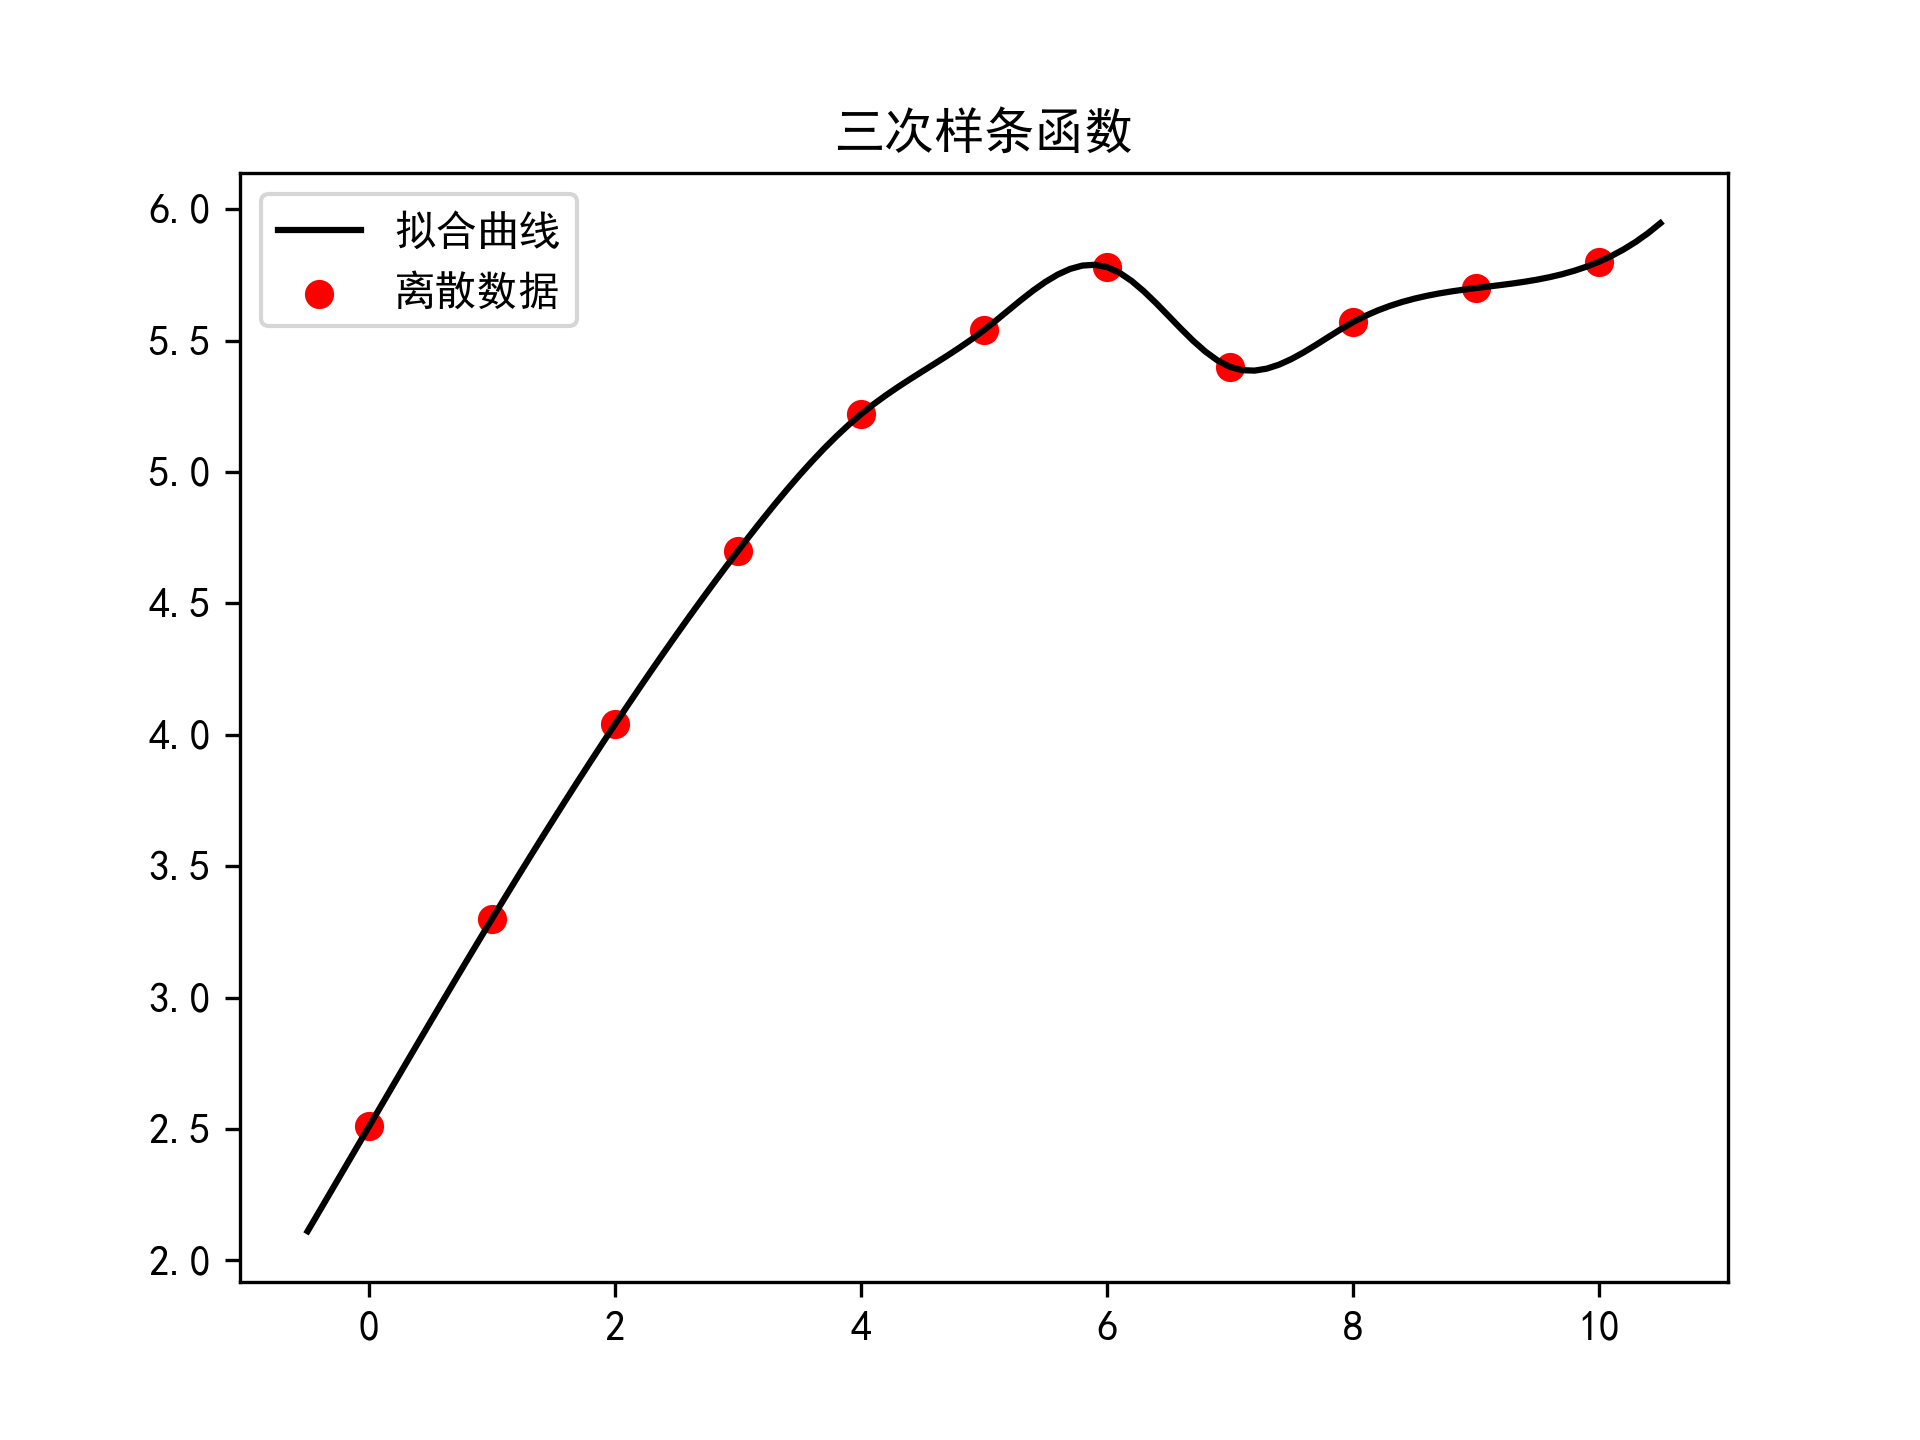
\includegraphics[width=\textwidth]{spline}
      \caption{三次样条插值图像}
      \label{fig:spline}
\end{figure}


\subsection{结论}

\begin{enumerate}[(1)]
    \item 编写程序实现了第一型边界条件和第二型边界条件下的三次样条插值计算;
    \item 三次样条插值得到的函数二阶导数连续,因此其光滑性较好;
    \item 目前算法使用的是待定系数法求解,当插值节点较多时,计算量较大,应加以改进。
\end{enumerate}

\clearpage
\section{离散数据的最佳平方逼近}


% chapter chapter1 (end)